\subsection{MÔ HÌNH ĐỘNG HỌC PHÂN TỬ VỀ CẤU TẠO CHẤT}
\Binhluan{
\subsubsection{Nội dung mô hình động học phân tử về cấu tạo chất}	
\begin{itemize}
\item Các chất được cấu tạo từ các hạt riêng biệt là các phân tử.
\item Các phân tử chuyển động không ngừng. Chuyển động của các phân tử được gọi là \textbf{chuyển động nhiệt}.
\item Các phân tử chuyển động càng nhanh thì nhiệt độ của vật do chúng tạo nên càng cao.
\item Giữa các phân tử có lực hút và lực đẩy, gọi chung là lực liên kết phân tử.
\end{itemize}
\begin{note}
Thuật ngữ phân tử trong mô hình trên được dùng để chỉ chung các hạt cấu tạo chất: phân tử, nguyên tử, ion.
\end{note}
}{
Chuyển động hỗn loạn, không ngừng của các hạt rất nhỏ dưới tác dụng của các phân tử chất lỏng hoặc chất khí được gọi là chuyển động Brown.
\begin{center}
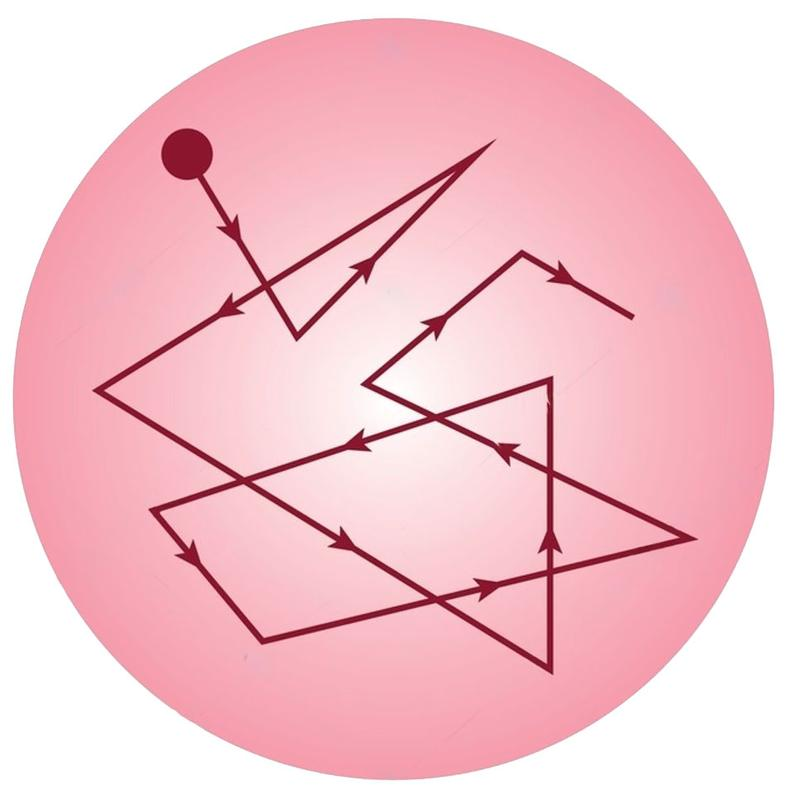
\includegraphics[width=4cm]{Images/brown}
\end{center}
}

\begin{center}
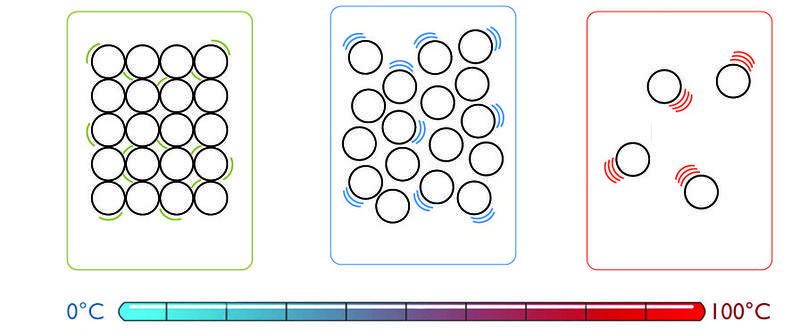
\includegraphics[width=8cm]{Images/cautaochat}
\end{center}
\subsubsection{Lực liên kết phân tử}
Giữa các phân tử có lực hút và lực đẩy, gọi chung là \textbf{lực liên kết phân tử}.
\begin{itemize}
\item Nếu khoảng cách giữa các phân tử rất nhỏ (cỡ kích thước phân tử): Lực đẩy lớn hơn lực hút.
\item Nếu khoảng cách giữa các phân tử lớn hơn kích thước phân tử: Lực hút lớn hơn lực đẩy.
\item Nếu khoảng cách giữa các phân tử rất lớn (so với kích thước phân tử): Lực liên kết không đáng kể.
\end{itemize}
\subsection{CẤU TRÚC CỦA CHẤT RẮN, CHẤT LỎNG VÀ CHẤT KHÍ}
\setcounter{paragraph}{0}
\subsubsection{Các thể rắn, lỏng, khí}
\begin{center}
	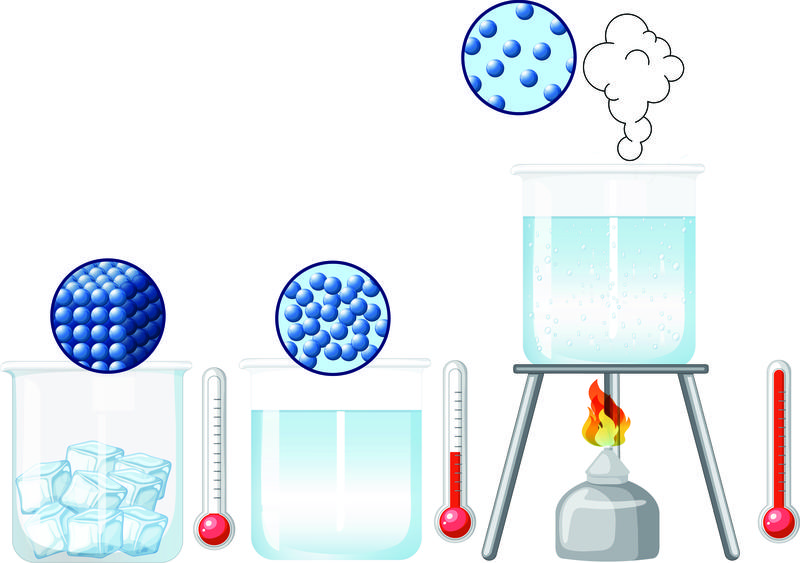
\includegraphics[width=8cm]{Images/phantu2}
\end{center}
\immini{	
\subsubsection{Sơ lược cấu trúc của chất rắn}
\begin{itemize}
\item Trong chất rắn, các phân tử ở rất gần nhau.
\item Lực tương tác giữa các phân tử chất rắn rất mạnh.
\end{itemize}}{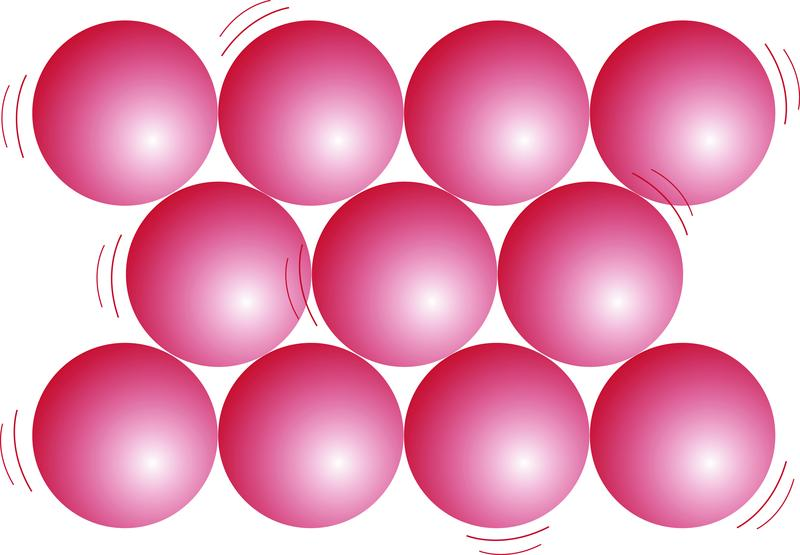
\includegraphics[width=4cm]{Images/chatran1}}
\noindent\faSignIn~\textbf{Hệ quả:}
\begin{itemize}
\item Các phân tử chất rắn được giữ ở các vị trí cân bằng và mỗi phân tử chỉ có thể dao động xung quanh vị trí cân bằng xác định này.
\item Các chất ở thể rắn có thể tích và hình dạng xác định.
\end{itemize}
\Binhluan{\faTags~\textbf{Phân loại:}\par
\begin{itemize}
\item Chất rắn kết tinh: Có cấu trúc tinh thể, các phân tử liên kết chặt với nhau và sắp xếp theo một trật tự hình học xác định, tuần hoàn trong không gian, gọi là mạng tinh thể. Muối ăn, kim cương, hầu hết kim loại,... là những chất rắn kết tinh.
\item Chất rắn kết tinh có hai loại là chất rắn đơn tinh thể và chất rắn đa tinh thể:
\end{itemize}
}{Cùng một chất nhưng cấu trúc tinh thể khác nhau thì tính chất vật lí cũng rất khác nhau. Ví dụ như than chì và kim cương.}
\begin{itemize}
\item []
\begin{itemize}
\item[+] Chất rắn đơn tinh thể: Mạng tinh thể được được lặp lại về cấu trúc và hướng trong toàn khối tinh thể.
\item[+] Chất rắn đa tinh thể: Gồm nhiều khối đơn tinh thể liên kết hỗn độn với nhau.
\end{itemize}
\end{itemize}
\begin{center}
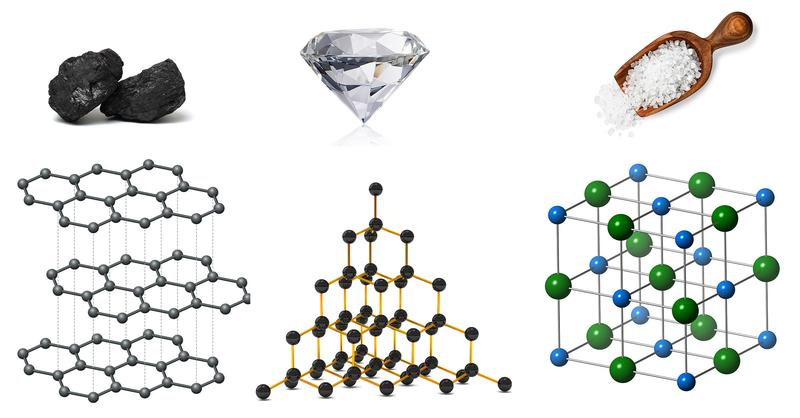
\includegraphics[width=8cm]{Images/chatrankettinh}
\begin{center}		
\textit{Cấu trúc tinh thể của than chì, kim cương và muối ăn}
\end{center}
\end{center}

\begin{itemize}
\item[] 
\begin{itemize}
\item Chất rắn vô định hình: Không có cấu trúc tinh thể.\\ 
Thuỷ tinh, nhựa đường, cao su,... là những chất rắn vô định hình.
\end{itemize}\end{itemize}

\subsubsection{Sơ lược cấu trúc của chất lỏng}
\immini{
\begin{itemize}
\item Trong chất lỏng, các phân tử ở xa nhau hơn so với các phân tử trong chất rắn.
\item  Lực tương tác giữa các phân tử chất lỏng nhỏ hơn trong chất rắn.
\end{itemize}
}{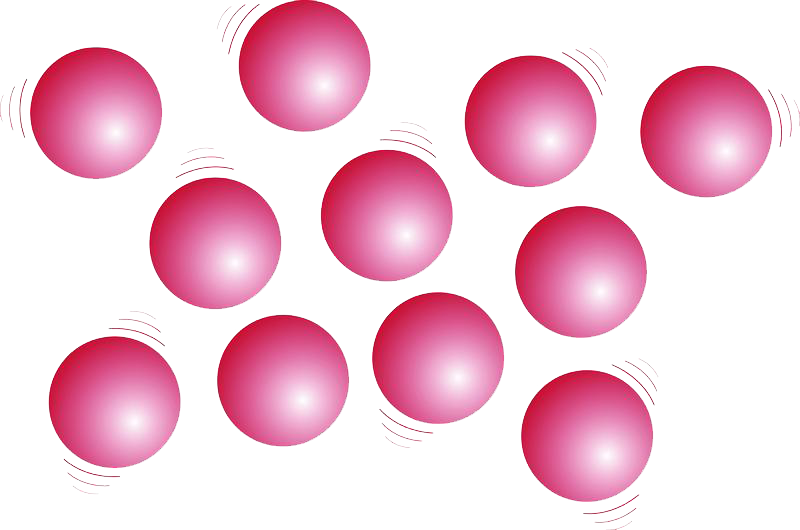
\includegraphics[width=4cm]{Images/chatlong}}
\faSignIn~ \textbf{Hệ quả:}
\begin{itemize}
\item Các phân tử dao động xung quanh các vị trí cân bằng và các vị trí cân bằng này lại có thể thay đổi.
\item Các chất ở thể lỏng có thể tích xác định nhưng không có hình dạng riêng mà có hình dạng của phần bình chứa nó.
\end{itemize}
\subsubsection{Sơ lược cấu trúc của chất khí}
\immini{\begin{itemize}
\item Trong chất khí, các phân tử ở xa nhau hơn so với các phân tử trong chất lỏng. 
\item Khoảng cách giữa các phân tử rất lớn so với kích thước của chúng
\item Lực tương tác giữa các phân tử hầu như không đáng kể (trừ khi va chạm nhau).
\end{itemize}}{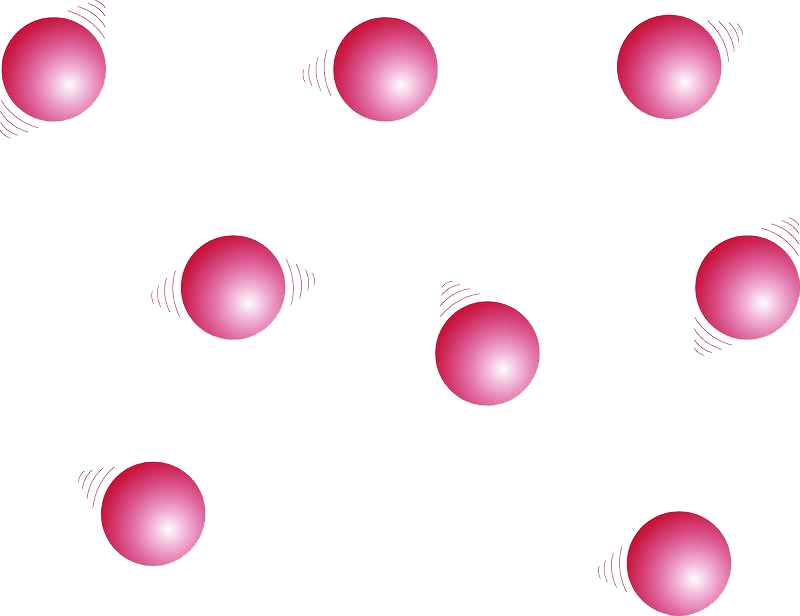
\includegraphics[width=4cm]{Images/chatkhi}}
\faSignIn~\textbf{Hệ quả:}
\begin{itemize}
\item Các phân tử khí chuyển động hỗn loạn, không ngừng về mọi phía.
\item Các chất ở thể khí không có thể tích và hình dạng riêng mà có thể tích và hình dạng của bình chứa.
\end{itemize}	
\subsubsection{Thể Plasma}
\newghichu{Ở thể này chất không tồn tại dưới dạng các nguyên tử, phân tử mà tồn tại dưới dạng các ion và các electron tự do.}
\begin{center}
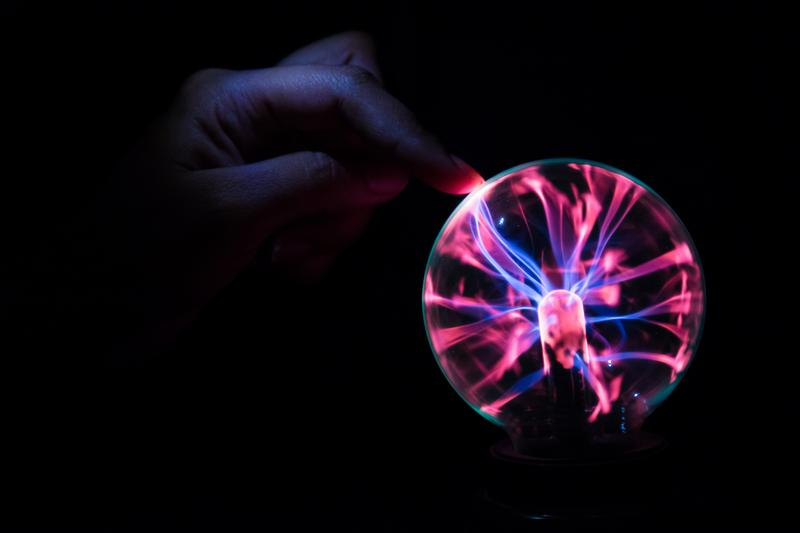
\includegraphics[width=8cm]{Images/close-up-hands}
\end{center}
\begin{bang}[tabularx=p{3cm}|X|X|X]{So sánh đặc điểm của chất ở các thể}
\textbf{Thể}&\quad \quad \quad \textbf{Rắn}&\quad \quad \quad \textbf{Lỏng}&\quad \quad \quad \textbf{Khí}\\
&\quad \quad 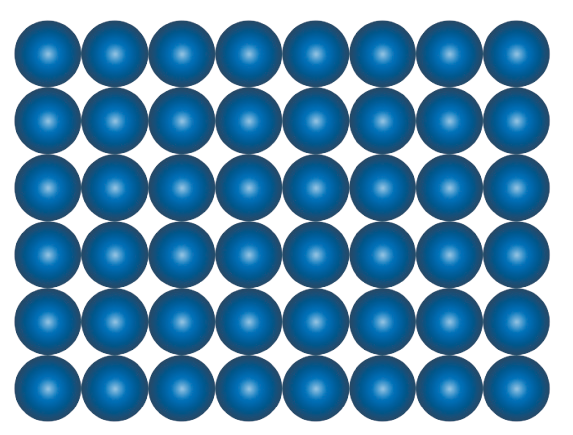
\includegraphics[width=2cm]{Images/ran3}& \quad \quad 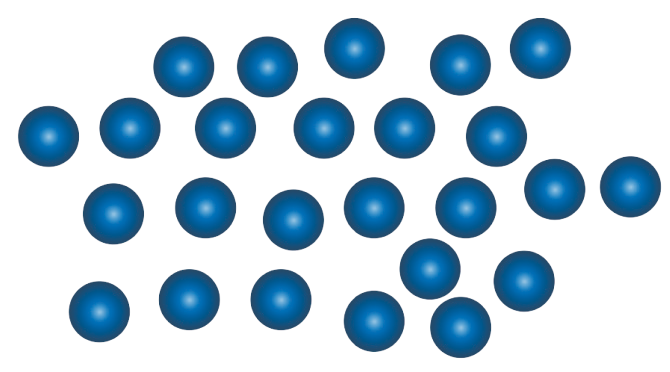
\includegraphics[width=2cm]{Images/long3}& \quad \quad 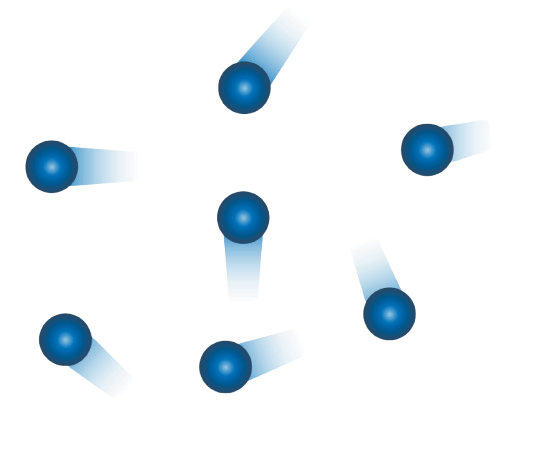
\includegraphics[width=2cm]{Images/khi3}\\\hline
%&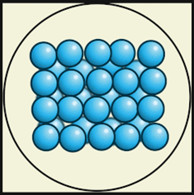
\includegraphics[width=1cm]{Images/ran} &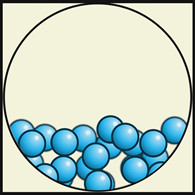
\includegraphics[width=1cm]{Images/long}&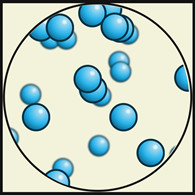
\includegraphics[width=1cm]{Images/khi} \\\hline
\textbf{Khoảng cách giữa các phân tử}&Rất gần &Xa hơn khoảng cách giữa các phân tử chất rắn &Rất lớn so với kích thước phân tử  \\\hline
\textbf{Lực liên kết phân tử}&Rất mạnh &Yếu hơn liên kết giữa các phân tử chất rắn &Rất yếu \\\hline
\textbf{Chuyển động phân tử}& Dao động quanh vị trí cân bằng xác định
\vspace{-\baselineskip}
\begin{center}
\begin{tikzpicture}[scale=.3,thick,>=stealth']
\tkzDefPoints{0/0/o}
\draw[fill=Mapcolor, very thick, Mapcolor] (o) circle(1cm);
\draw[->, dashed, Mapcolor] (0,1) -- (0,2);
\draw[->, dashed, Mapcolor]  (0.75,0.75) -- (1.5,1.5);
\draw[->, dashed, Mapcolor]  (1,0) -- (2,0);
\draw[->, dashed, Mapcolor]  (-0.75,0.75) -- (-1.5,1.5);
\draw[->, dashed, Mapcolor]  (-1,0) -- (-2,0);
\draw[->, dashed, Mapcolor]  (-0.75,-0.75) -- (-1.5,-1.5);
\draw[->, dashed, Mapcolor]  (0,-1) -- (0,-2);
\draw[->, dashed, Mapcolor]  (0.75,-0.75) -- (1.5,-1.5);
\end{tikzpicture}
\end{center}&Dao động quanh vị trí cân bằng có thể di chuyển 
\vspace{-\baselineskip}
\begin{center}
\begin{tikzpicture}[scale=.3,thick,>=stealth']
\tkzDefPoints{0/0/o}
\draw[fill=blue, very thick, Mapcolor] (o) circle(1cm);
\draw[->, dashed, Mapcolor] (0,1) -- (0,2);
\draw[->, dashed, Mapcolor]  (0.75,0.75) -- (1.5,1.5);
\draw[->, dashed, Mapcolor]  (1,0) -- (2,0);
\draw[->, dashed, Mapcolor]  (-0.75,0.75) -- (-1.5,1.5);
\draw[->, dashed, Mapcolor]  (-1,0) -- (-2,0);
\draw[->, dashed, Mapcolor]  (-0.75,-0.75) -- (-1.5,-1.5);
\draw[->, dashed, Mapcolor]  (0,-1) -- (0,-2);
\draw[->, dashed, Mapcolor]  (0.75,-0.75) -- (1.5,-1.5);
\draw[->, dashed, Mapcolor] (1.1,-0.2) .. controls (2.8,-0.2) and (3.75,-1) .. (4,-2.5);
\begin{scope}[shift={(4,-3.75)},rotate=-20]
\tkzDefPoints{0/0/o}
\draw[dashed,very thick, Mapcolor] (o) circle(1cm);
\draw[->, dashed, Mapcolor] (0,1) -- (0.1161,2.1006);
\draw[->, dashed, Mapcolor]  (0.75,0.75) -- (1.5,1.5);
\draw[->, dashed, Mapcolor]  (1,0) -- (2,0);
\draw[->, dashed, Mapcolor]  (-0.75,0.75) -- (-1.5,1.5);
\draw[->, dashed, Mapcolor]  (-1,0) -- (-2,0);
\draw[->, dashed, Mapcolor]  (-0.75,-0.75) -- (-1.5,-1.5);
\draw[->, dashed, Mapcolor]  (0,-1) -- (0,-2);
\draw[->, dashed, Mapcolor]  (0.75,-0.75) -- (1.5,-1.5);
\end{scope}
\end{tikzpicture}
\end{center}&Chuyển động hỗn loạn
\vspace{-\baselineskip}
\begin{center}
\begin{tikzpicture}[scale=.3,thick,>=stealth']
\tkzDefPoints{0/2.5/o', 0/0/o, 2.6/-3/a, 0/-4.5/b}
\draw[fill=Mapcolor, very thick, Mapcolor] (o) circle(.5cm);
\draw[dashed,Mapcolor,->] (0.4,-0.5) -- (2.2,-2.6);
\draw[dashed,Mapcolor] (a) circle(.5cm);
\draw [dashed,Mapcolor,->](2.1,-3.3) -- (0.5,-4.2);
\draw [dashed,Mapcolor](b) circle(.5cm);
\draw[dashed,Mapcolor,->] (0.6,-4.5) -- (3.6,-4.5);
\end{tikzpicture}
\end{center}\\\hline
\textbf{Khả năng nén}&Rất khó nén &Rất khó nén &Dễ nén \\\hline
\textbf{Hình dạng}&Xác định &Phụ thuộc bình chứa &Theo hình dạng bình chứa \\
&\begin{center}
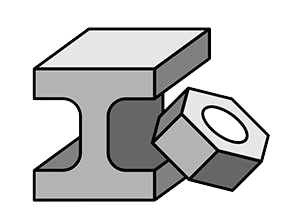
\includegraphics[width=2cm]{Images/chatran2}
\end{center}&\begin{center}
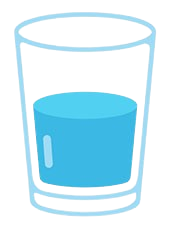
\includegraphics[width=1.1cm]{Images/chatlong2}
\end{center}&\begin{center}

\includegraphics[width=1.5cm]{Images/chatkhi2}
\end{center} \\\hline
\textbf{Thể tích}&Xác định&Xác định&Phụ thuộc bình chứa 
\end{bang}